\chapter{Conceptual Design}
Following the clarification of the task is the conceptual design, where in this section of the product development process, designers engage in creative exploration and evaluation of various design ideas and concepts.

Pahl and Beitz describe conceptual design as the phase of the design process where the essential problems are identified through abstraction, function structures are established, appropriate working principles are sought, and these elements are combined to form a working structure. This process lays down the foundation for the solution path by elaborating on a solution principle, ultimately specifying the principle solution. \cite{Pahl07d}

Figure \ref{} shows the steps involved in the conceptual design phase.


\section{Abstraction}
Traditional solution principles or designs may not provide optimal answers in the presence of new technologies, procedures, materials, and scientific discoveries. Preconceptions, conventions, and risk aversion often hinder unconventional but better and more cost-effective solutions. To overcome fixation on conventional ideas, designers utilize abstraction, focusing on the general and essential aspects rather than particular details. By formulating the task appropriately, the overall function and essential constraints become clear, enabling objective solution selection. \cite{Pahl07b}

To help in identification of the essential problems, following abstraction techniques are used:
\begin{itemize}
    \item Step 1 - Eliminate personal preferences.
    \item Step 2 - Omit requirements that have no direct bearing on the function and the essential constraints.
    \item Step 3 - Transform quantitative into qualitative data and reduce them to essential
          statements.
    \item Step 4 - As far as it is purposeful, generalise the results of the previous step.
    \item Step 5 - Formulate the problem in solution-neutral terms. \cite{Pahl07c}
\end{itemize}

Figure \ref{} shows the result of the abstraction process.

\section{Function Structures}
In the design process, a function refers to a specific action or purpose that a product or system should fulfill. It captures the essence of what the product or system is intended to do, focusing on the desired outcomes rather than specific solutions or components. Functions serve as the building blocks of a design, providing a clear understanding of the overall purpose and functionality of the intended product or system.

The function structure is a graphical representation of the functions of a system and their interrelationships. It is a hierarchical representation of the functions of a system, starting with the overall function and breaking it down into sub-functions. The function structure is a useful tool for identifying the essential functions of a system and for identifying the relationships between the functions. \cite{Pahl07e}

Figure \ref{} shows the representation of the function structure and the process of breaking down the overall function into sub-functions.


\subsection{Overall Function}
Based on the result of abstraction, the overall function of the system can be represented and visualized using a function structure diagram. This diagram, as shown in Figure \ref{}, shows the overall function, which will be broken down into sub-functions in the next step.

\subsection{Sub-Functions}
Subsequently, after the abstraction process, the overall function is further decomposed into several sub-functions. This division is guided by the function structure, which represents the interconnections and dependencies between the functions. By analyzing the main flow of the system and considering the desired outcomes, the sub-functions are identified and organized within the function structure.

The purpose of this decomposition is to reduce the complexity of the overall system and facilitate the identification of suitable solution principles that can fulfill the required functions. By breaking down the main function into smaller, more manageable sub-functions, designers can focus on addressing specific aspects of the system's functionality and finding appropriate design solutions for each sub-function.

It is important to note that a simple and straightforward structure is desirable in the function structure. Such simplicity often leads to the development of uncomplicated and cost-effective systems. By keeping the structure of the function hierarchy straightforward and easy to understand, the design process can be streamlined, and potential complexities can be minimized.

\section{Developing Working Principles}

In the process of developing working structures, one crucial step is to search for working principles. Working principles refer to the physical effects and characteristics that fulfill specific functions of the structure being designed. These principles are combined to create the working structure, and they encompass both the physical processes and the form design features.

The search for working principles aims to generate several potential solution variants, creating what is known as a solution field. This can be achieved by varying the physical effects and form design features. Often, multiple physical effects are involved in fulfilling a single subfunction or even multiple function carriers. \cite{Pahl07f}

In developing working principles, there are multiple available methods in idea generation. These methods are categorized into three groups:

\begin{itemize}
    \item Conventional methods
    \item Intuitive methods
    \item Discursive methods
\end{itemize}

Conventional methods involve a systematic and data-driven approach. Designers gather information from various sources, such as literature, trade publications, and competitor catalogs, to stay informed about advancements and best practices. They analyze natural systems and existing technical systems to draw inspiration and identify opportunities for improvement. Analogies are used to substitute analogous problems or systems, leading to fresh perspectives. Additionally, empirical studies, such as measurements and model tests, provide tangible data for validating designs and predicting real-world performance. \cite{Pahl07g}

On the other hand, intuitive methods tap into creativity and associative thinking. Brainstorming fosters a collaborative environment where diverse perspectives generate a wide range of ideas without judgment. Method 635 adds structure to brainstorming, allowing for systematic idea development within a group. The Gallery Method combines individual work with group discussions, using sketches or drawings to explore solution proposals visually. Synectics involves combining apparently unrelated concepts to trigger new and fruitful ideas. \cite{Pahl07h}

Discursive methods provide systematic step-by-step procedures influenced by intuition and creativity. They involve deliberate analysis of physical processes, leading to multiple solution variants derived from the relationships between variables. This approach fosters a deeper understanding of the problem space, encouraging the discovery of novel solutions while maintaining a level of systematic rigor, making them effective for communication and collaboration among design teams. \cite{Pahl07i}

\subsection{Searching for Working Principles}
To find working principles, the following methods discussed in Section 3.2 were
applied:

methods \dots
methods \dots
methods \dots

text and images \dots

\subsection{Selecting Working Principles}

As can be seen in Figure \ref{}, multiple working principles were generated. Each of these working principles can be combined to form a working structure and hence a wide range of solutions are available. However, not all of these solutions are feasible and practical. The task of evaluating each of the solution will consumed a lot of time and resources.


It is necessary to reduce the vast number of theoretically possible but practically unachievable solutions as early as possible. However, caution should be exercised not to discard valuable working principles, as they often play a crucial role in forming a favorable and effective working structure when combined with others.


Although there is no entirely foolproof method, employing a systematic and verifiable selection process significantly simplifies the task of selecting promising solutions from numerous proposals. This selection process consists of two steps: elimination and preference. Initially, all clearly unsuitable proposals are removed. If a substantial number of solutions still remain, preference is given to those that stand out as markedly superior. Only these preferred solutions are evaluated during the final stages of the conceptual design phase.

Pahl and Beitz suggest the following criteria for eliminating unsuitable solutions:
\begin{itemize}
    \item Compatible with the overall task (Criteria A)
    \item Fulfill demands of requirement list (Criteria B)
    \item Realisible in principle (Criteria C)
    \item Within permissible cost (Criteria D)
\end{itemize}

These criteria are applied step by step to examine each solution. If any of the exclusion criteria are not met, the solution is rejected, and further criteria are not assessed. Additionally to the exclusion criteria, the following preference criteria are used to prioritize the remaining solutions:

\begin{itemize}
    \item Incorporates direct safety measures (Criteria E)
    \item Preferred by the designer (Criteria F)
\end{itemize}

Criteria E to F are then used to prioritize solutions if there are still too many options after the initial screening. The remarks column provides explanations for excluding or favoring each solution. The final assessment of the functional principles is recorded in the rightmost column of the selection list.

image \dots

\section{Combination of Working Structures}

In this step, the working principles are combined to form working structures. The combination process is done with the help of Morphological Chart. The Morphological Chart is a tool that allows designers to systematically combine working principles to form working structures. It is a matrix that lists the working principles in the rows and the sub-functions in the columns. It is also important to note that the working principles are now updated based on the result from the selection process in chapter \ref{}.
In the following Figure 18, the developed Morphological Box is presented with the identified functional structures. Due to the high compatibility among the identified functional principles, numerous different functional structures can be formed.

\section{Firming Up into Principle Solution Variants}
DIRECT TRANSLATE !!


The understanding of the solutions resulting from the functional structures is still relatively abstract, and therefore, a selection or evaluation cannot be conducted yet. To increase the level of information, preferably quantitatively but at least qualitatively, sketches, simplified assumptions, visualization models, or preliminary experiments are utilized [Reference 25].

In this chapter, the identified functional structures are now specified into concrete solution variants and presented in accurately scaled hand sketches. The accompanying text provides a brief explanation of their operation, along with potential advantages and disadvantages. The information obtained serves as the basis for the subsequent selection process.

Due to the constraints related to the available space and the predetermined positioning of the packaging system, there are minimal geometric differences among the individual solution variants. Distinctions mainly pertain to the areas of "rotation," "conveyance," and "storage" of the bags.


\subsection{Solution Variant 1}
The first solution variant is based on the working structure shown in Figure 18.
Solution Variant 1 features a tablet-like design with components (Raspberry Pi, Battery, Camera, and Screen) arranged in a manner similar to that of a tablet device. The screen orientation is landscape, providing a wider display view. The device is meant to be held with a body grip for convenient handling.

\begin{figure}[ht!]
    \centering
    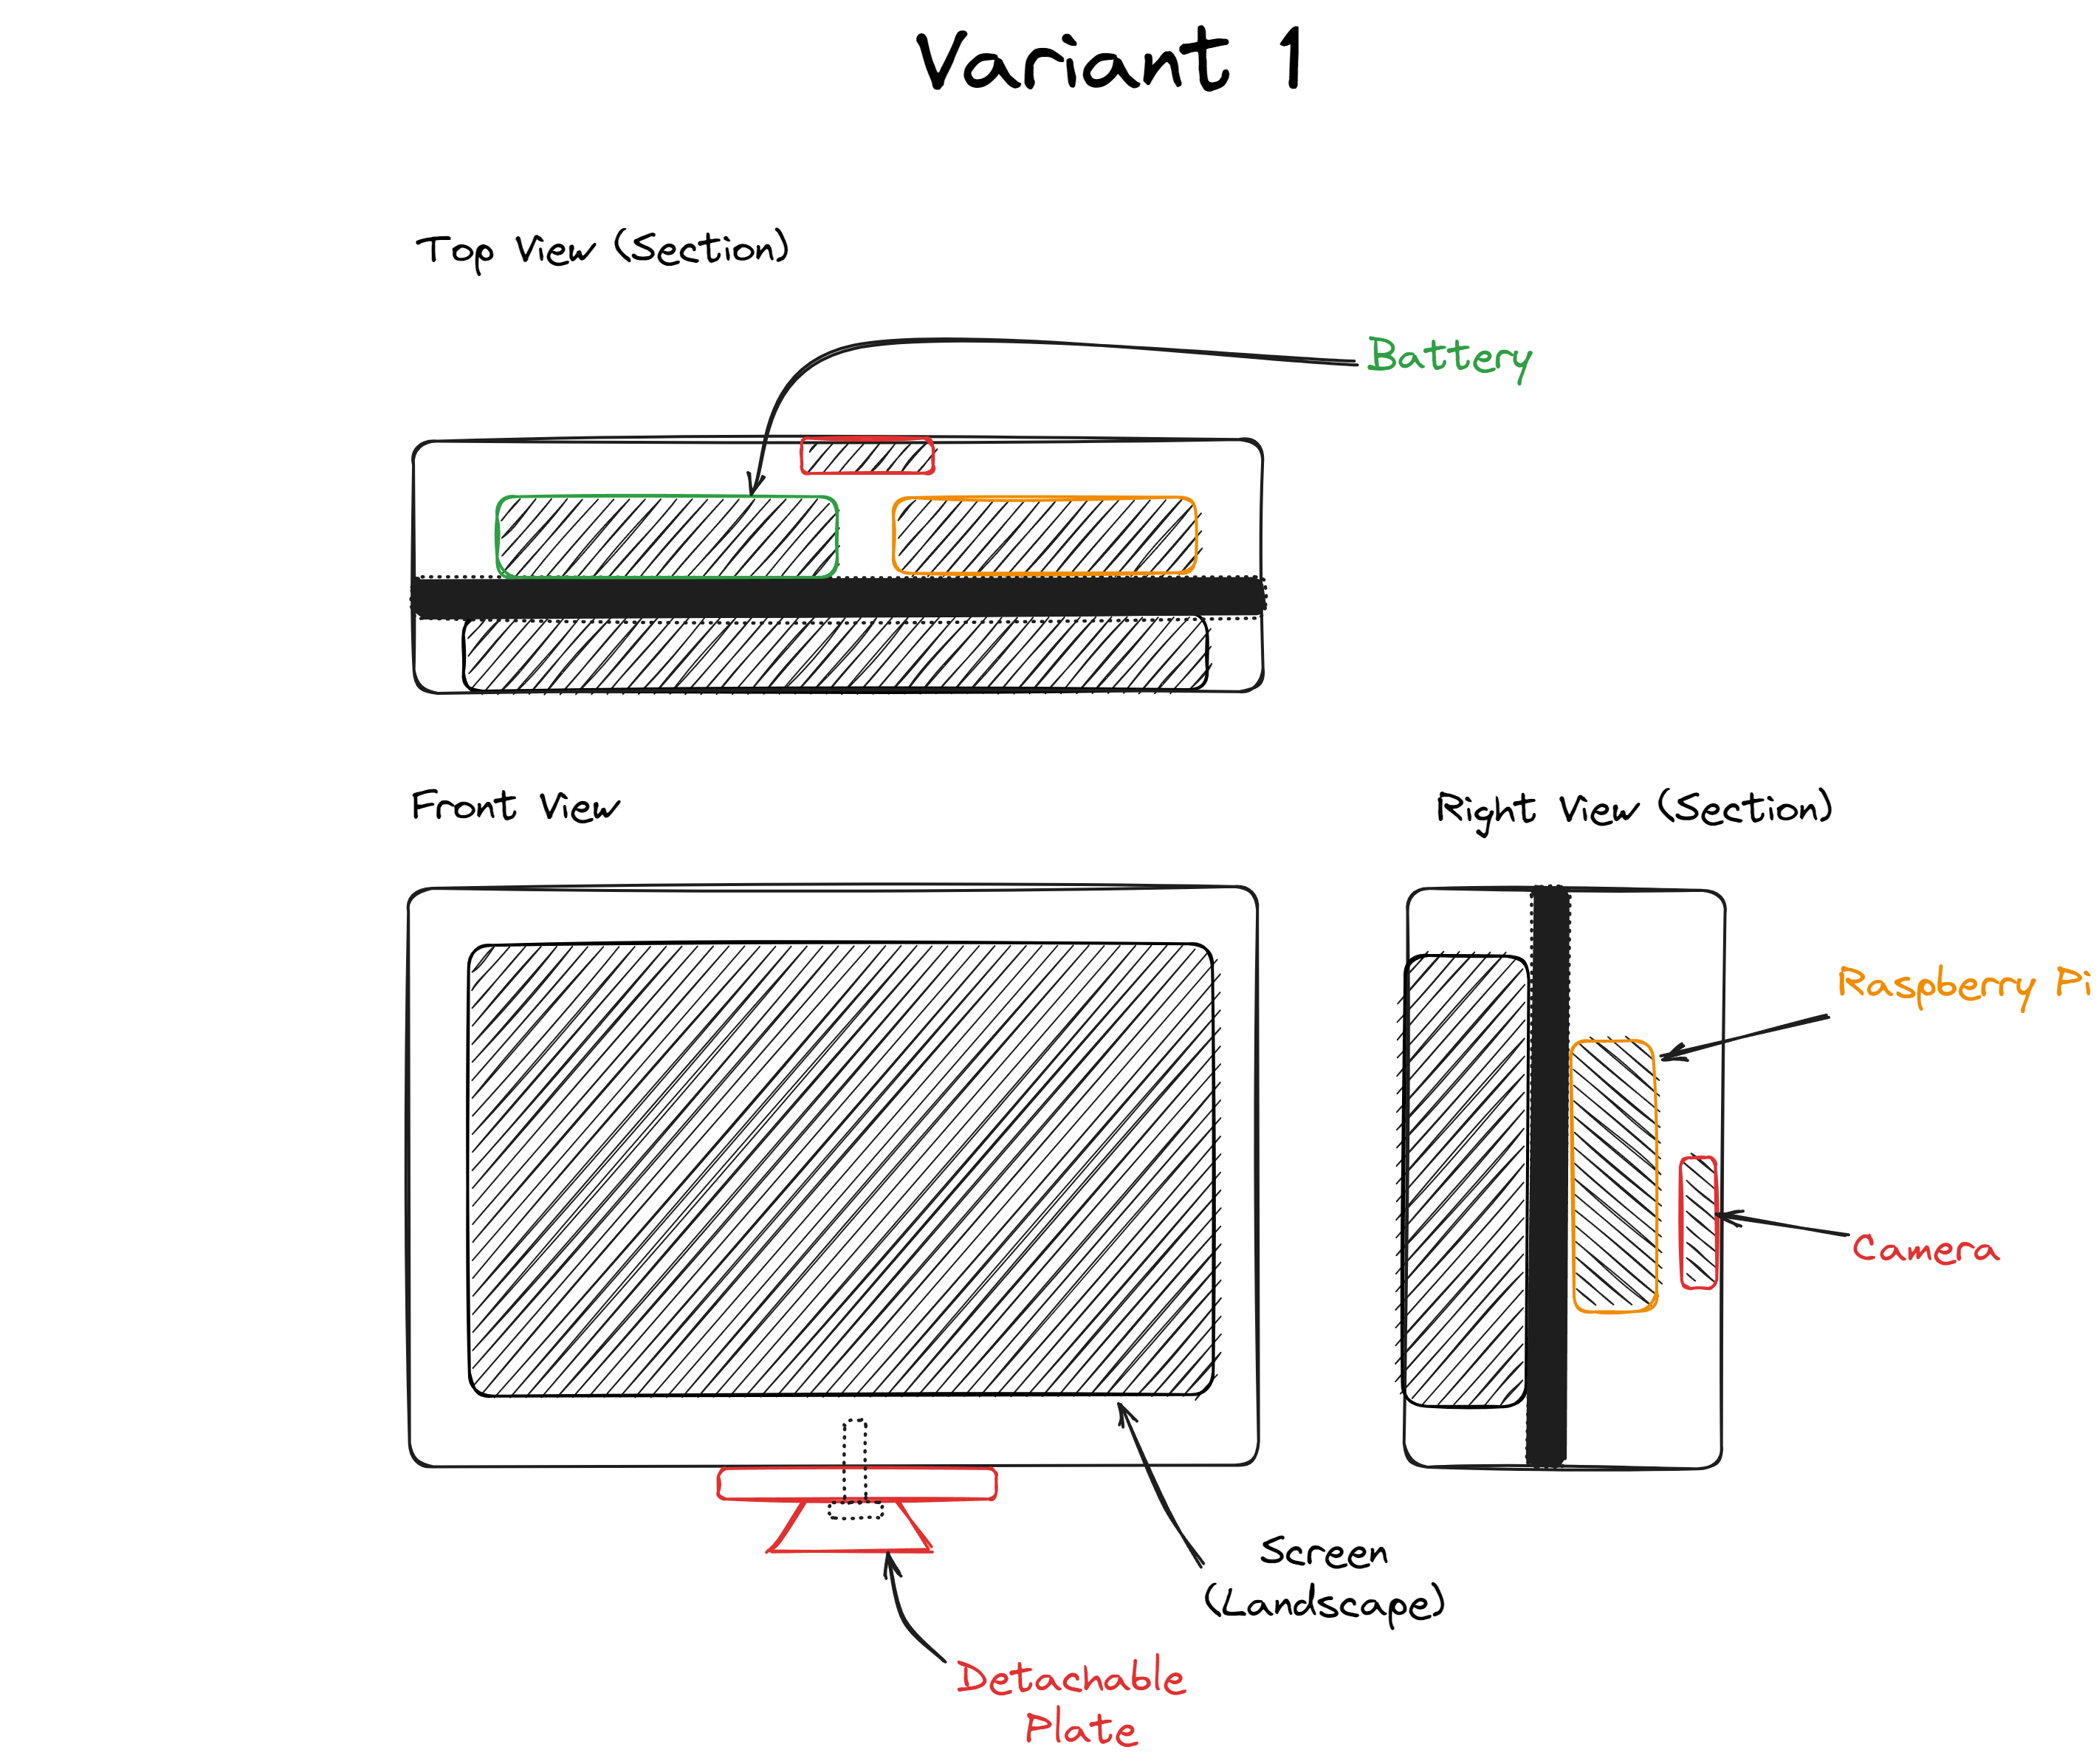
\includegraphics[width=\linewidth]{texs/Part1/chapter3/image/v1.png}
    \caption{Sketch of Solution Variant 1}
    \label{fig:sketch-solution-variant-1}
\end{figure}

The battery is fixed inside the device, ensuring a seamless and integrated appearance. The chassis type follows a sandwich structure, comprising a top cover, main body, and bottom cover, providing a robust and secure enclosure for the internal components.

For mounting purposes, a detachable plate tripod system is utilized, allowing easy attachment and removal of the device from a tripod stand. The primary control mechanism is a touch screen, enabling intuitive and user-friendly interactions with the device's functionalities.

\subsection{Solution Variant 2}
Solution Variant 2 shares a tablet-like design with Solution Variant 1, with components (Raspberry Pi, Battery, Camera, and Screen) arranged in a manner similar to a tablet device. However, it also incorporates features of a handheld console.

\begin{figure}[ht!]
    \centering
    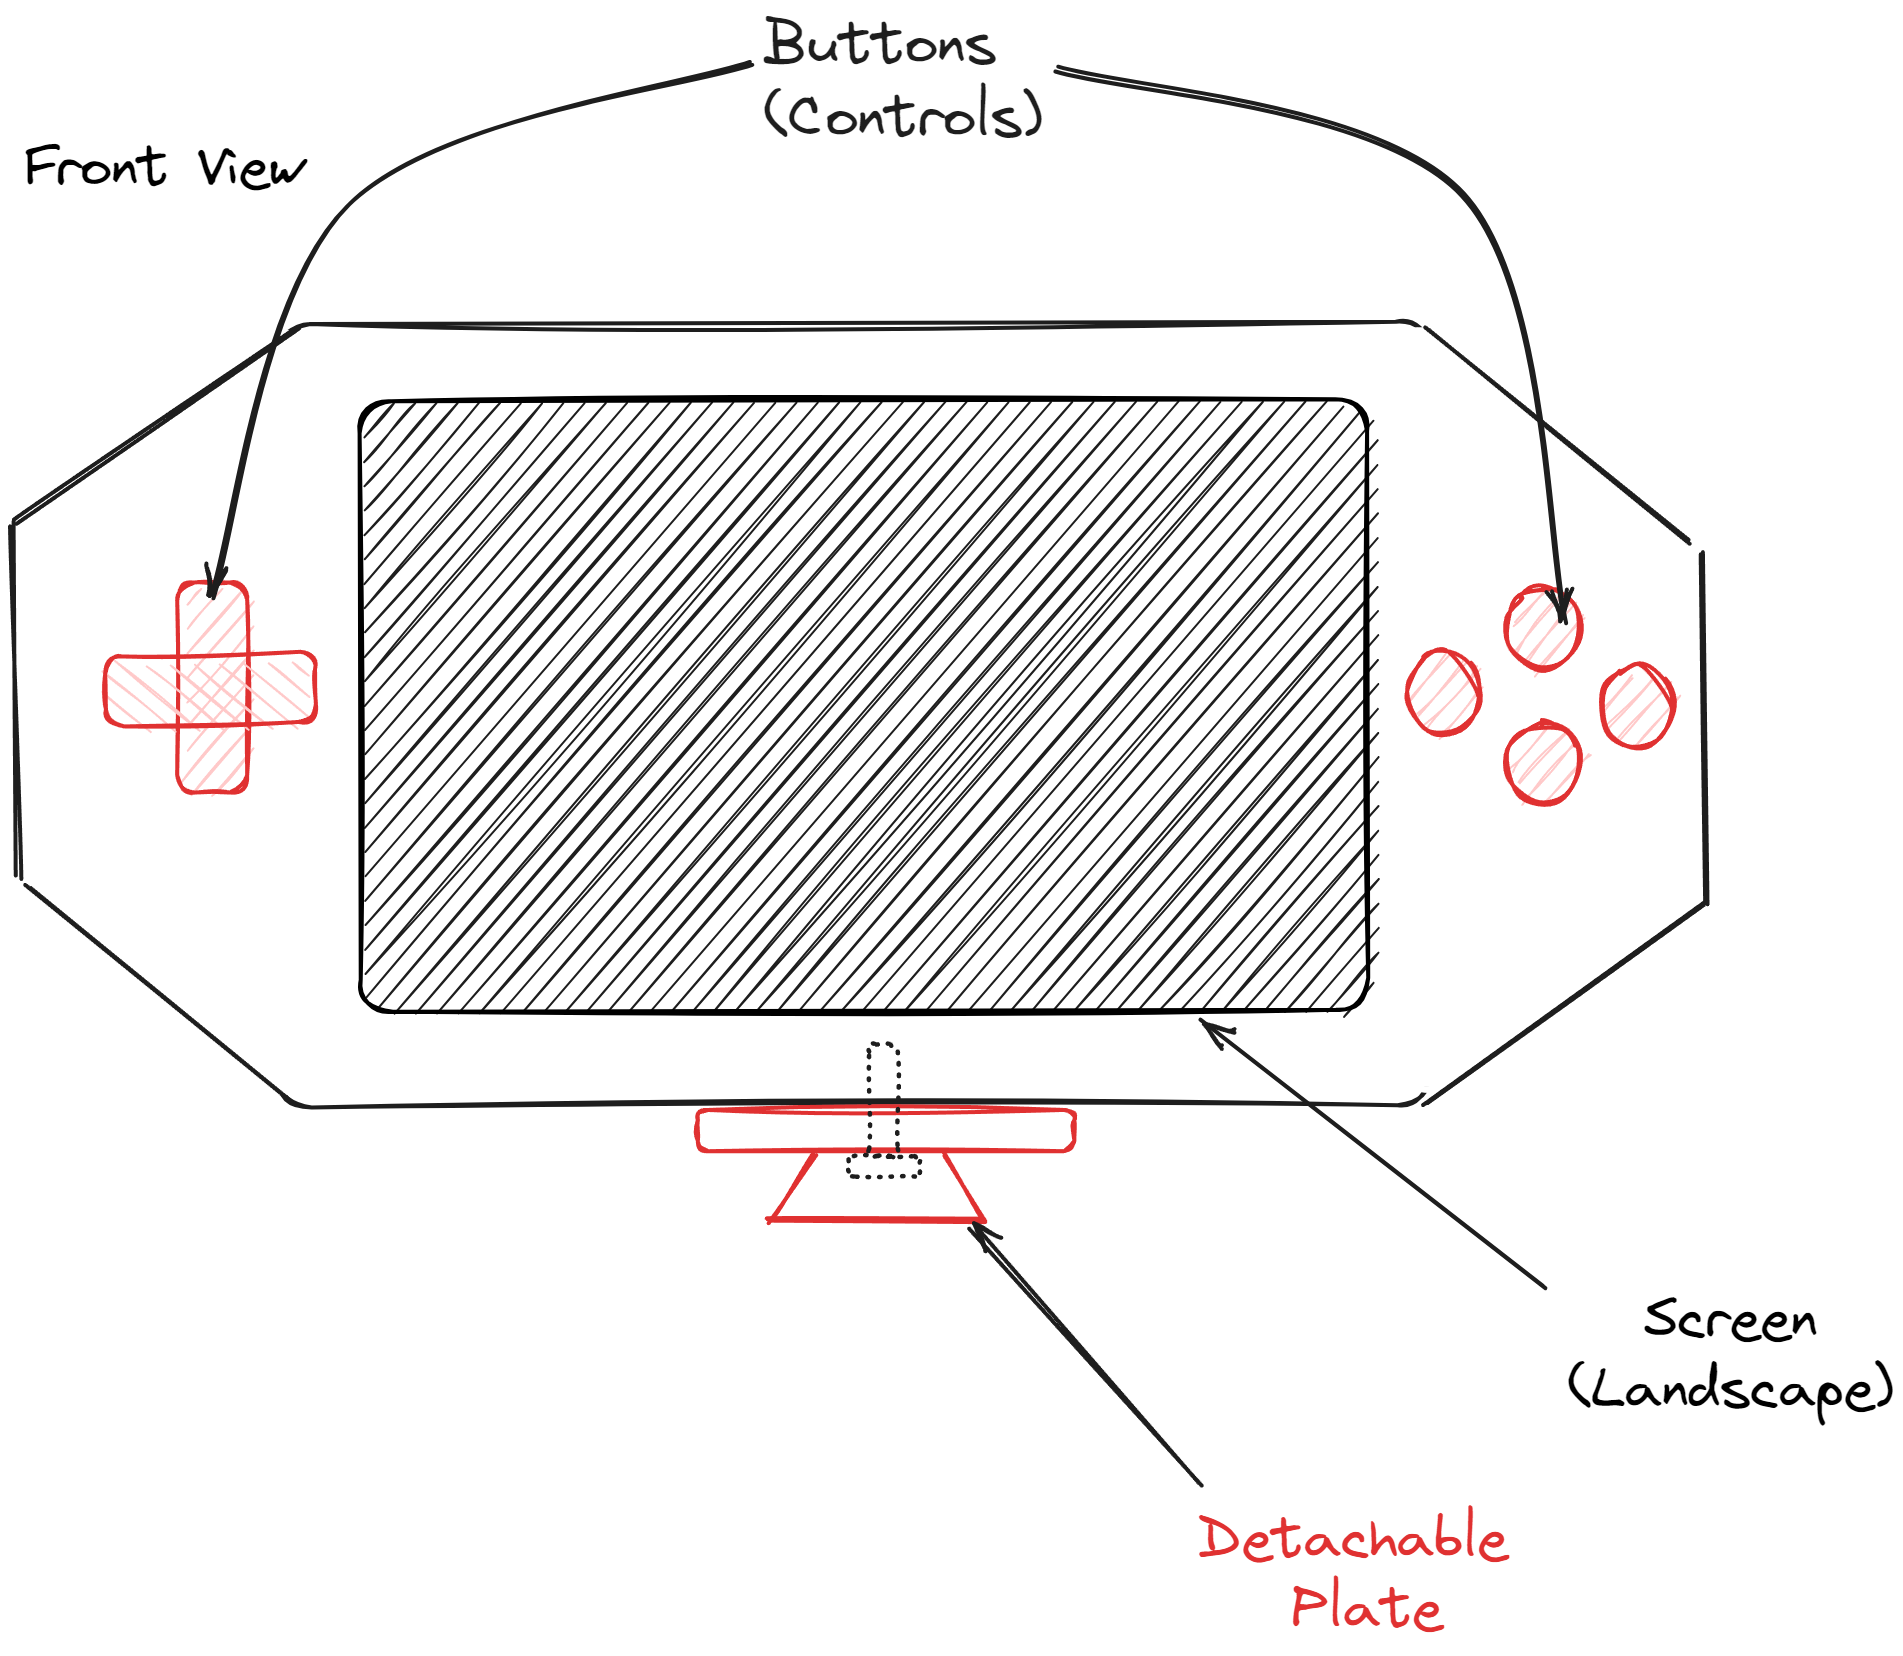
\includegraphics[width=\linewidth]{texs/Part1/chapter3/image/v2.png}
    \caption{Sketch of Solution Variant 2}
    \label{fig:sketch-solution-variant-2}
\end{figure}

The screen orientation remains in landscape mode, providing a wide display view. The device is meant to be held with a body grip, allowing comfortable handling.

While the battery is fixed inside the device, in this variant, it employs a battery pack instead of a built-in battery, possibly allowing for easier replacement and extended usage periods.

The chassis type continues to follow a sandwich structure, comprising a top cover, main body, and bottom cover, ensuring a sturdy and secure enclosure for the internal components.

Similar to Solution Variant 1, a detachable plate tripod system is used for mounting, facilitating easy attachment and removal from a tripod stand.

However, the control mechanism in Solution Variant 2 offers an added feature. In addition to the touch screen, it incorporates physical buttons, providing users with multiple input options for interactions with the device. This combination of touch screen and buttons enhances versatility and usability in various scenarios.

\subsection{Solution Variant 3}

Solution Variant 3 maintains the tablet-like component placement, with the Raspberry Pi, Battery, Camera, and Screen arranged in a similar manner as the previous variants. However, a significant difference is the screen orientation, which is now in portrait mode instead of landscape.

\begin{figure}[ht!]
    \centering
    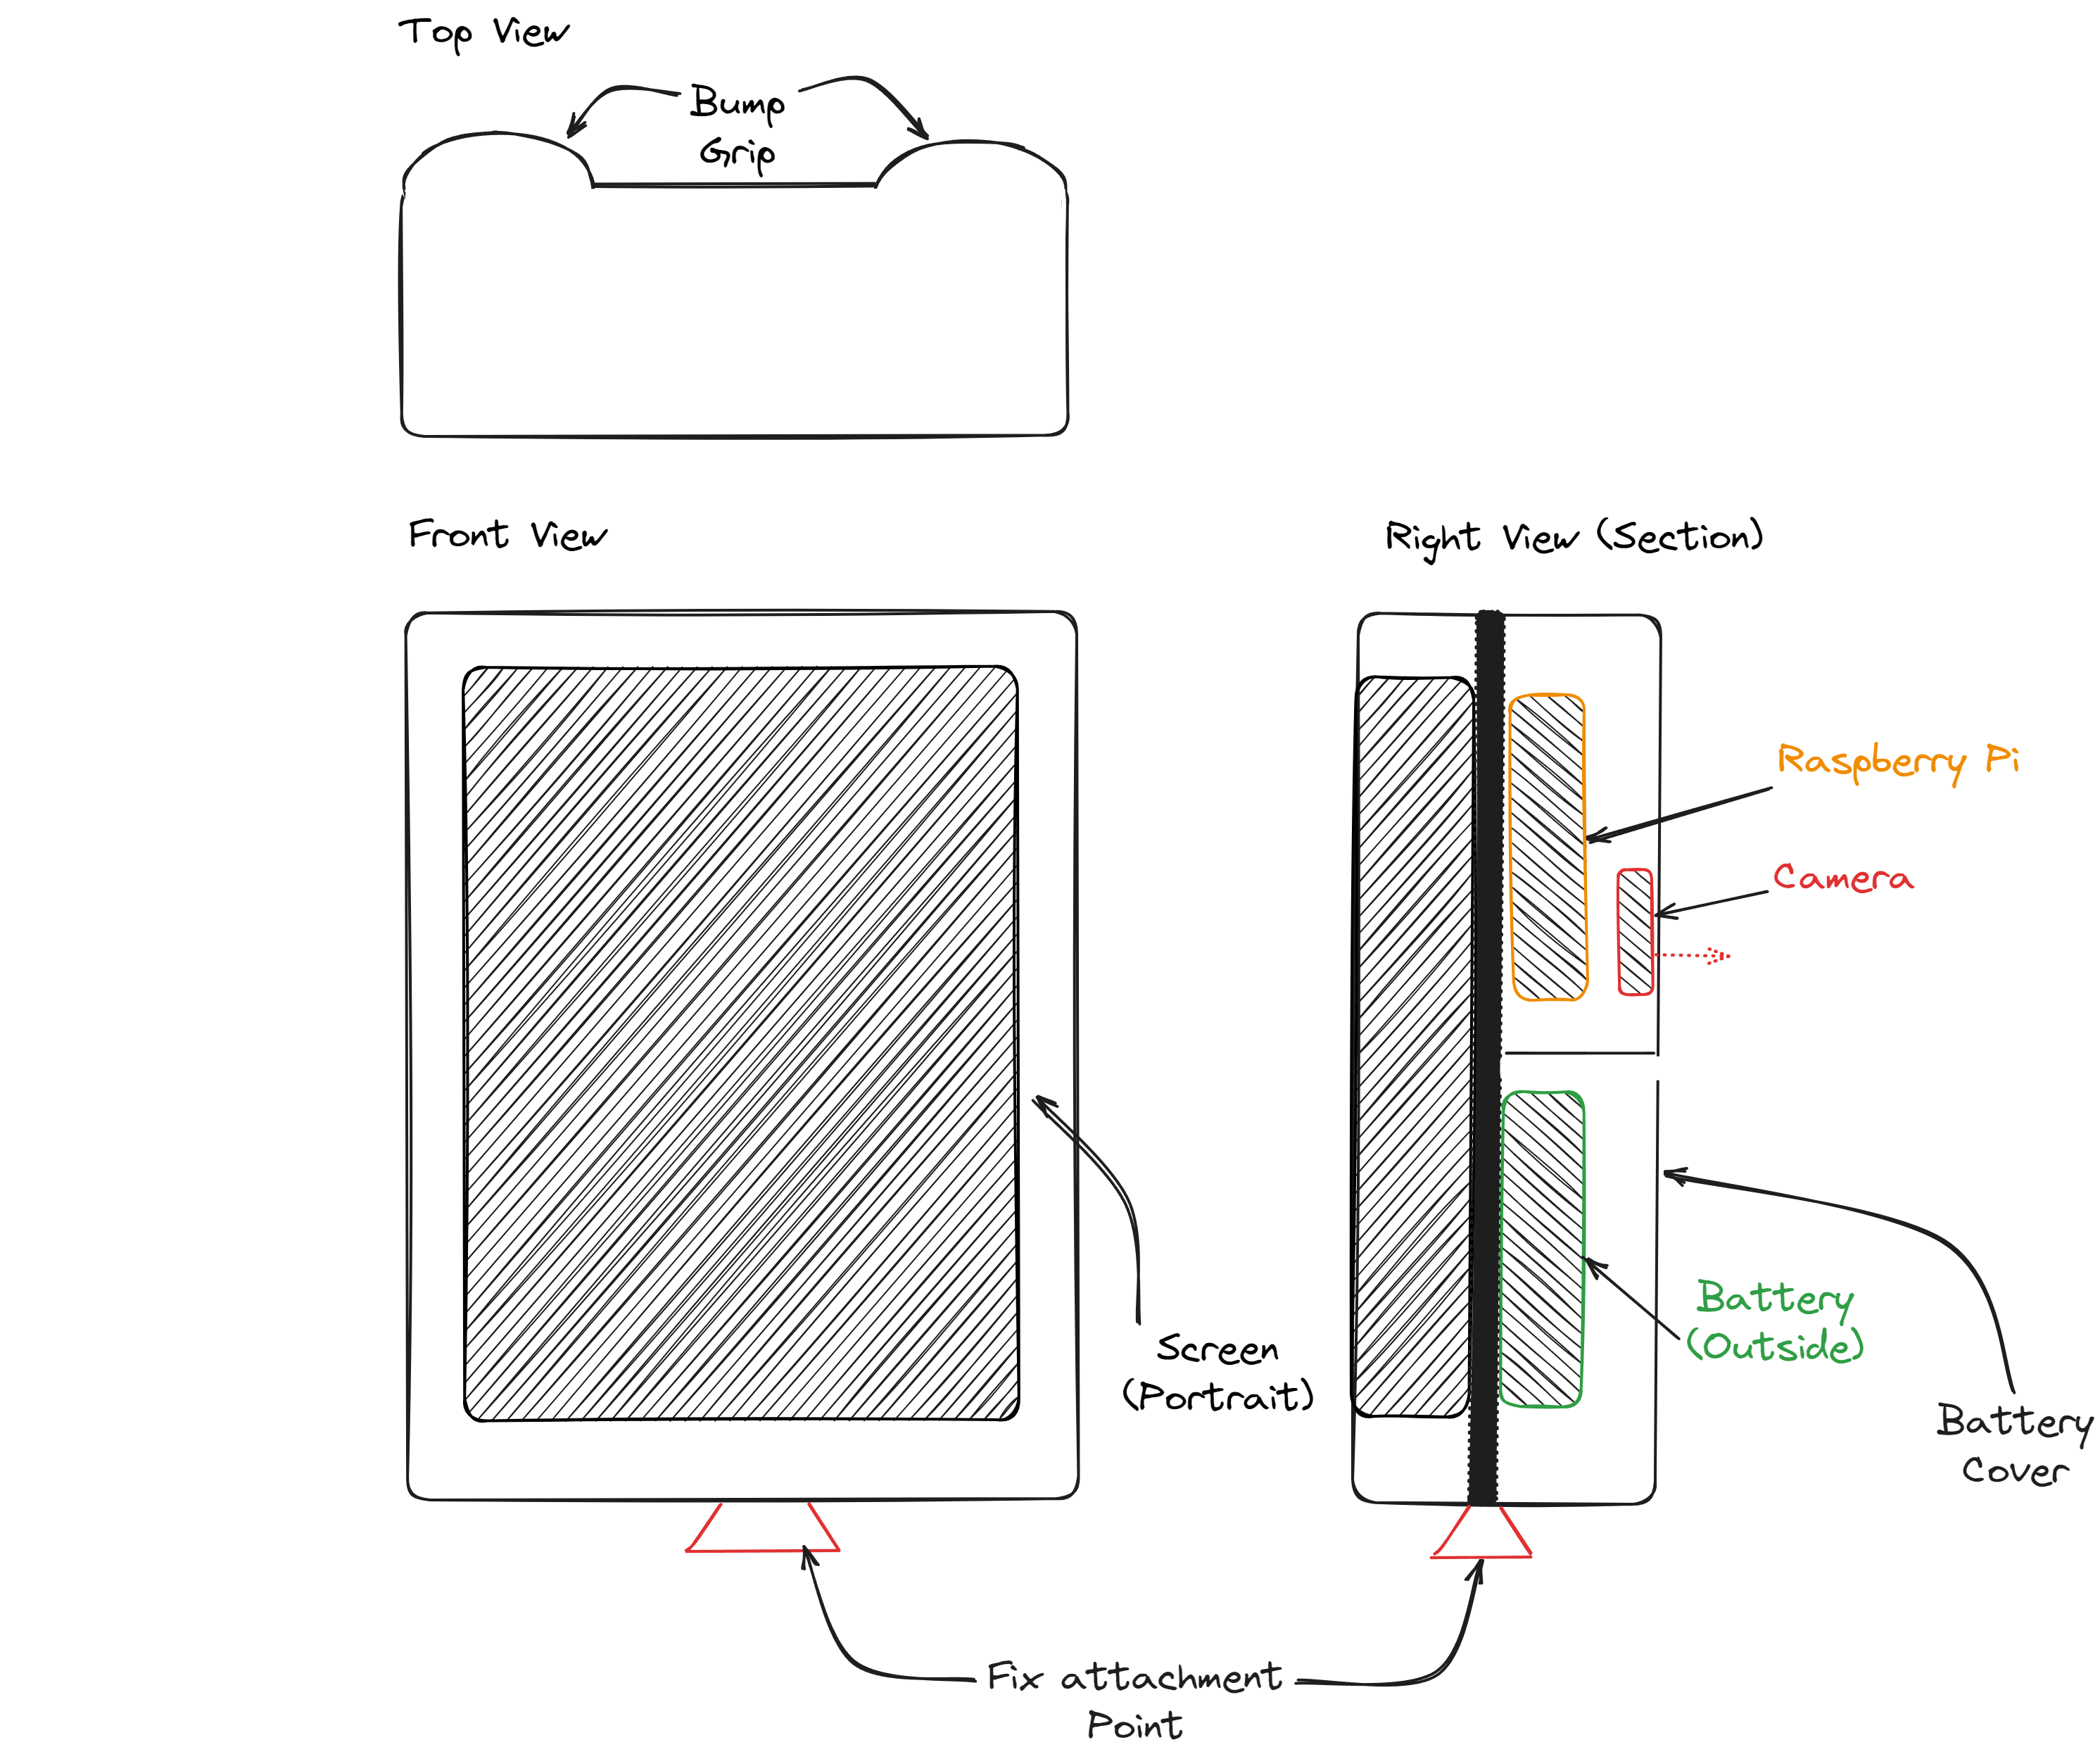
\includegraphics[width=\linewidth]{texs/Part1/chapter3/image/v3.png}
    \caption{Sketch of Solution Variant 3}
    \label{fig:sketch-solution-variant-3}
\end{figure}

With the portrait screen orientation, the device is designed to be held with a bump grip, offering a comfortable and secure way to handle the device in a vertical position.

Another change in this variant is the placement of the battery. Instead of being fixed inside the device, the battery is located externally. It is still in the form of a battery pack, but now positioned outside the main body.

Despite the changes, the chassis type remains a sandwich structure, comprising a top cover, main body, and bottom cover, ensuring robustness and protection for the internal components.

The mounting tripod system remains unchanged, using a detachable plate for easy attachment and detachment from a tripod stand.

The control mechanism in Solution Variant 3 continues to be a touch screen, providing intuitive and user-friendly interactions with the device's functionalities.

One advantage of the portrait screen orientation is the increased stability of the components, as the center of gravity is now aligned at the center of the device. This alignment may offer better balance and control when using the device in various orientations, enhancing its usability and versatility.

\subsection{Solution Variant 4}

Solution Variant 4 also features a tablet-like design, with the Raspberry Pi, Battery, Camera, and Screen components placed similarly to the previous variants. The screen orientation remains in portrait mode.

\begin{figure}[ht!]
    \centering
    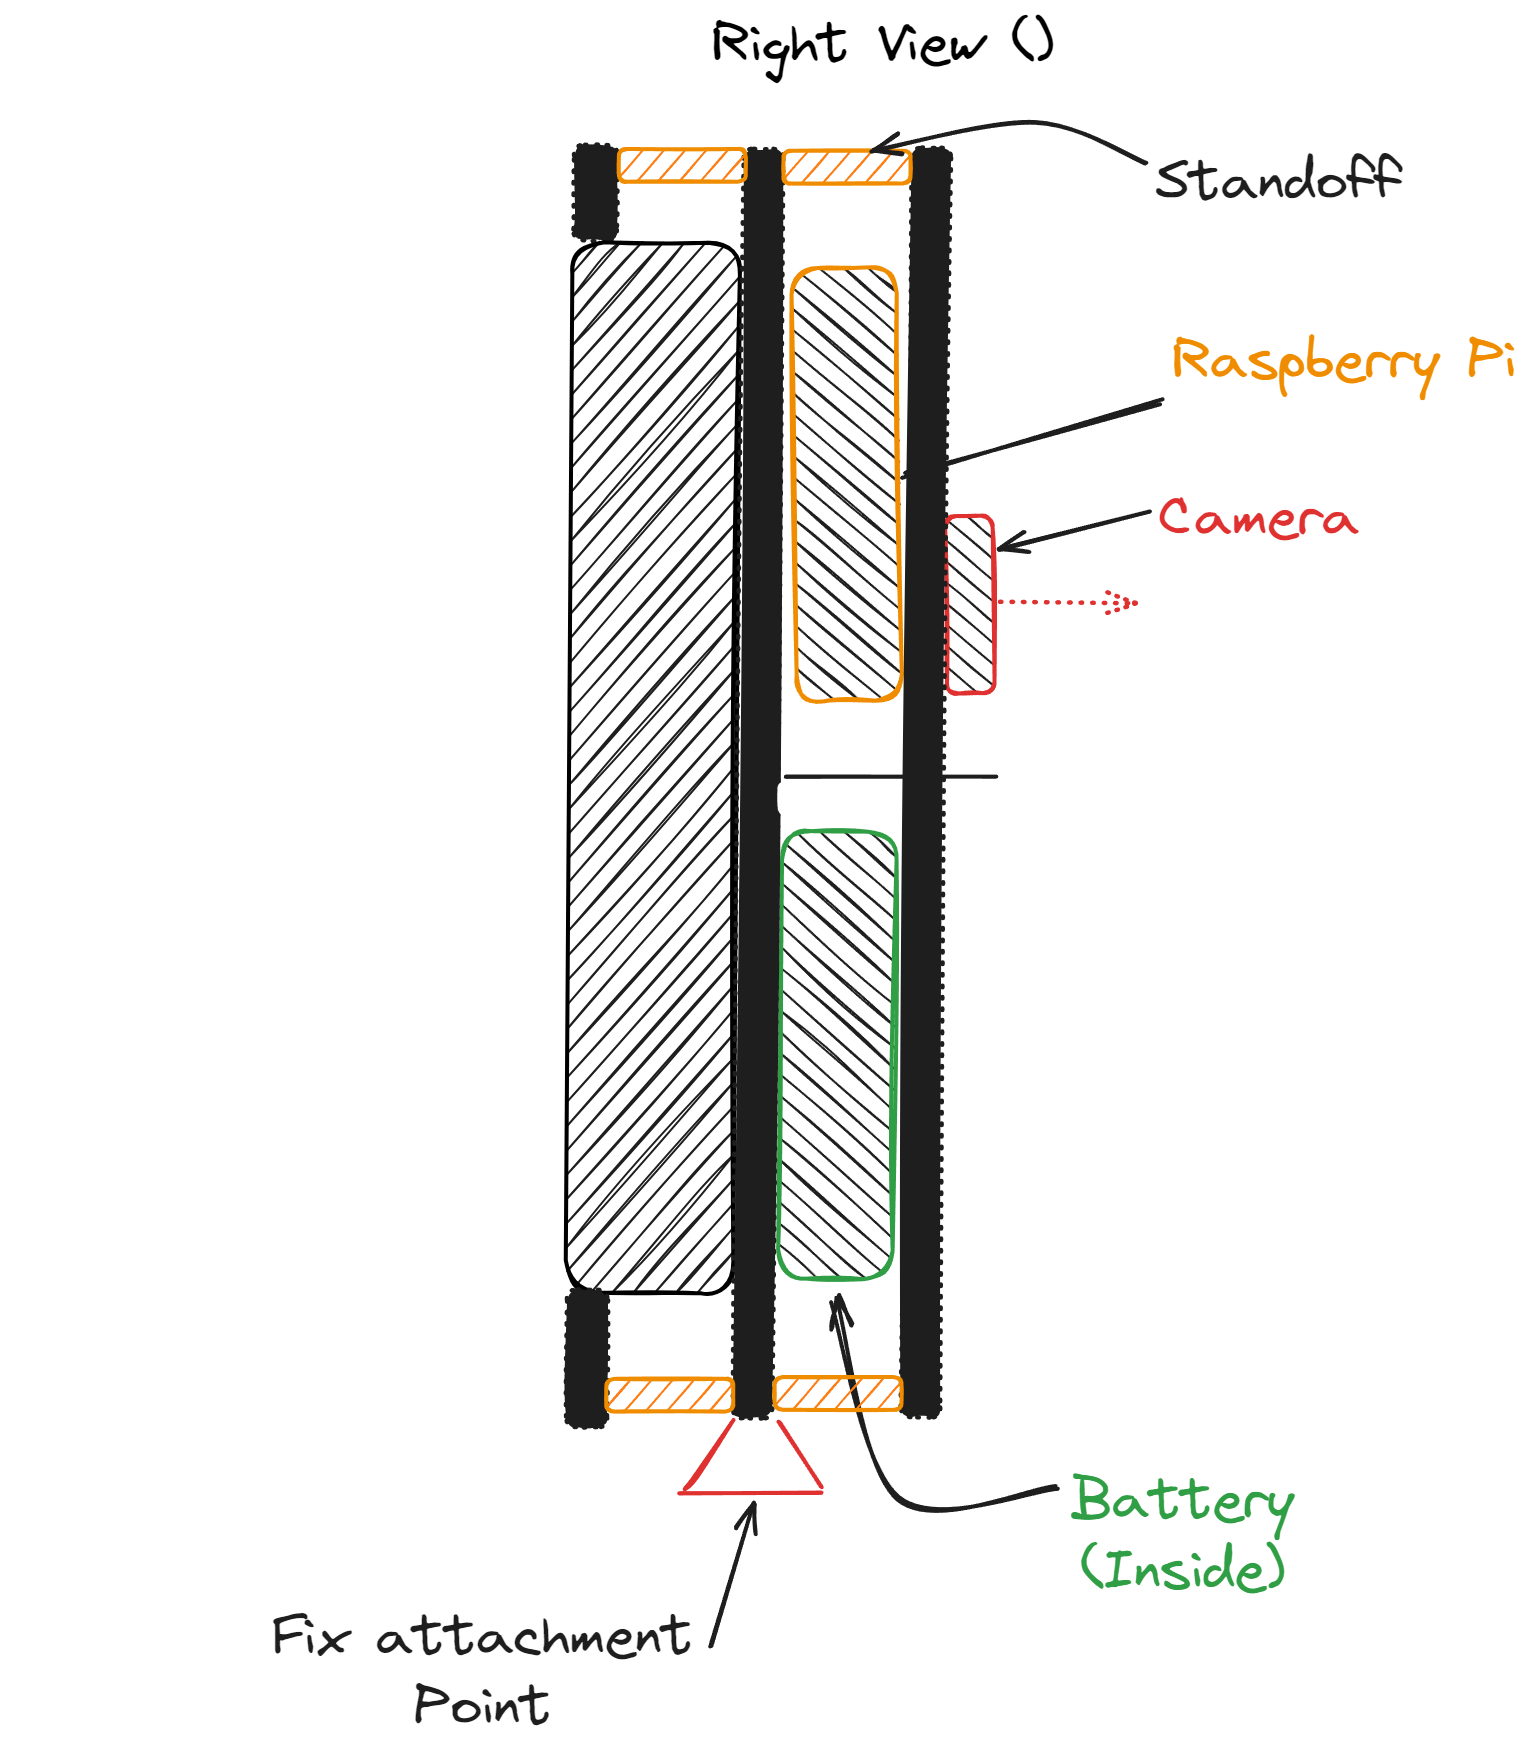
\includegraphics[scale=0.25]{texs/Part1/chapter3/image/v4.png}
    \caption{Sketch of Solution Variant 4}
    \label{fig:sketch-solution-variant-4}
\end{figure}


To ensure a secure and comfortable grip, the device is designed to be held with a bump grip, allowing users to handle it with ease.

In this variant, the battery is placed externally, and it takes the form of a power bank. This setup allows for convenient battery replacement or charging when needed.

The chassis type in Solution Variant 4 is different from the previous variants. It utilizes a skeleton design, with only the body layered and connected via standoffs. This lightweight and minimalistic chassis provides adequate support and protection for the internal components while reducing overall weight.

For mounting purposes, a fixed mounting plate is used, providing a stable attachment to a tripod stand.

The control mechanism remains consistent with the other variants, utilizing a touch screen for intuitive and user-friendly interactions with the device's functionalities.

\subsection{Solution Variant 5}

Solution Variant 5 introduces a different design approach with a Point of Service-like component placement. The Raspberry Pi, Battery, Camera, and Screen are arranged in a unique configuration where the screen is positioned at an angle, and the battery and Raspberry Pi are stacked on top of each other.

\begin{figure}[ht!]
    \centering
    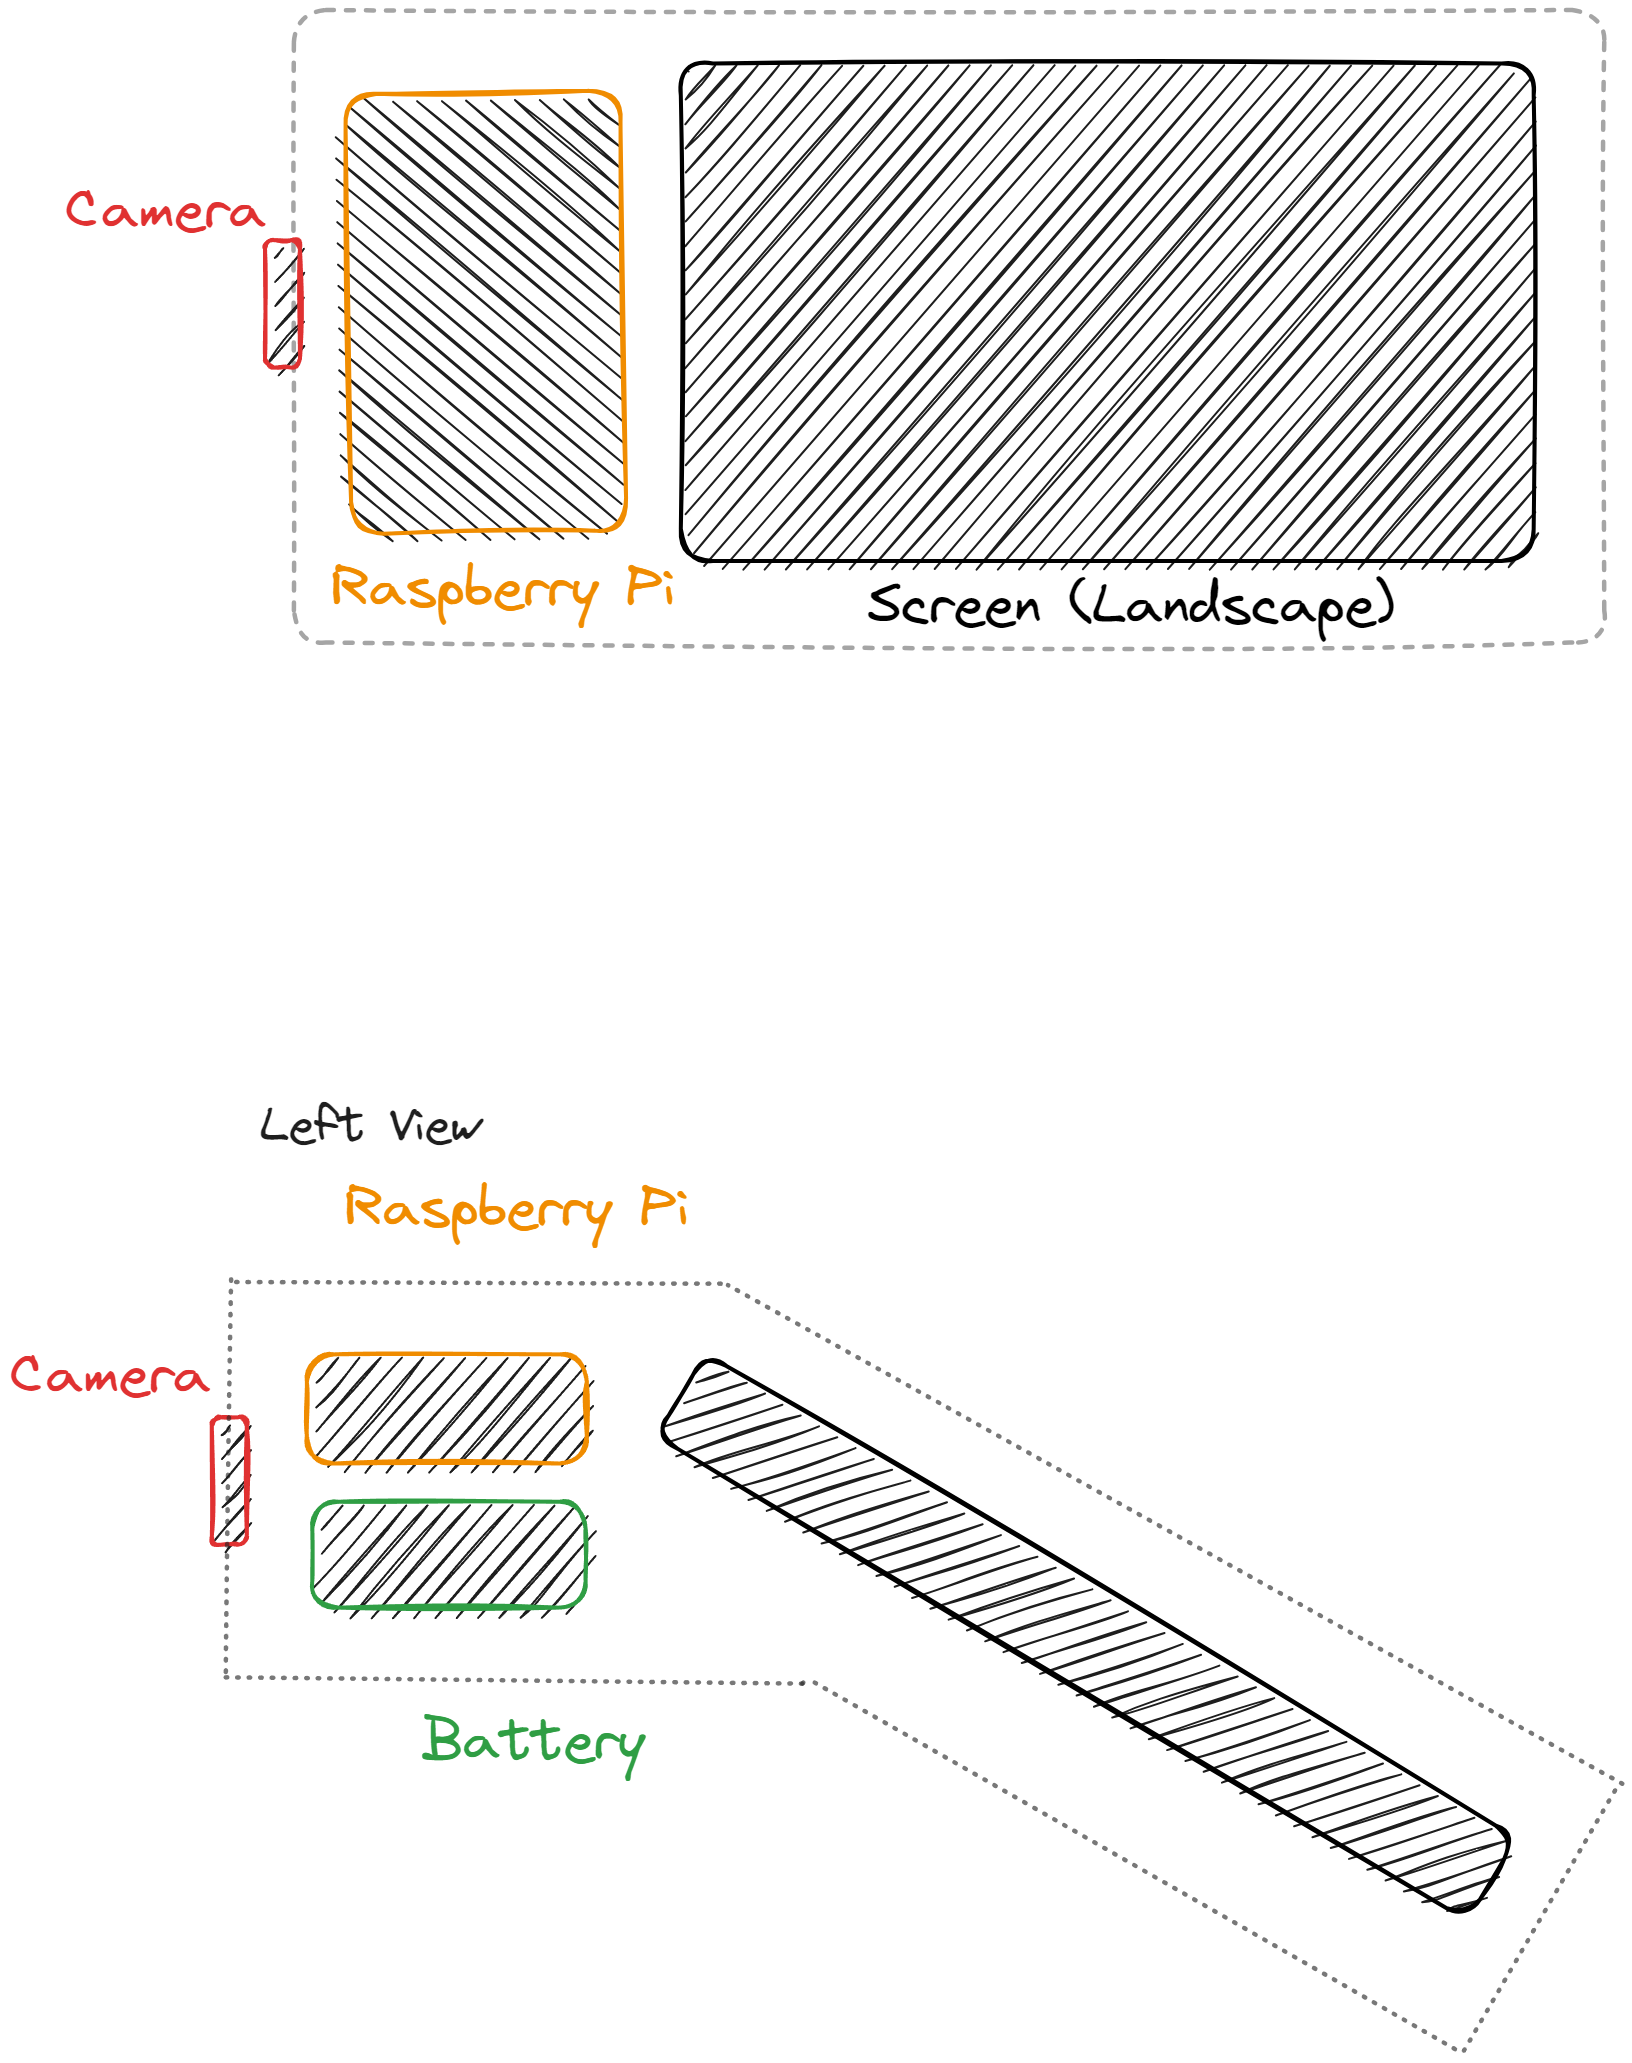
\includegraphics[scale=0.25]{texs/Part1/chapter3/image/v5.png}
    \caption{Sketch of Solution Variant 5}
    \label{fig:sketch-solution-variant-5}
\end{figure}

The screen orientation remains in portrait mode, providing a vertical display view.

For handling, the device is designed for a comfortable body grip, allowing users to securely hold and interact with the device.

In this variant, the battery is placed externally, and it utilizes AAA batteries with a battery holder. This setup offers the advantage of easy battery replacement and availability of standard batteries.

The chassis type follows a sandwich structure, consisting of a top cover, main body, and bottom cover, providing robustness and protection for the internal components.

The mounting tripod system is detachable, enabling easy attachment and detachment from a tripod stand.

Similar to the other variants, the control mechanism uses a touch screen, ensuring an intuitive and user-friendly interface for operating the device.

\subsection{Solution Variant 6}

Solution Variant 6 features a Point of Service-like component placement, where the Raspberry Pi, Battery, Camera, and Screen are arranged with the screen positioned at an angle, and the battery and Raspberry Pi are stacked together.

\begin{figure}[ht!]
    \centering
    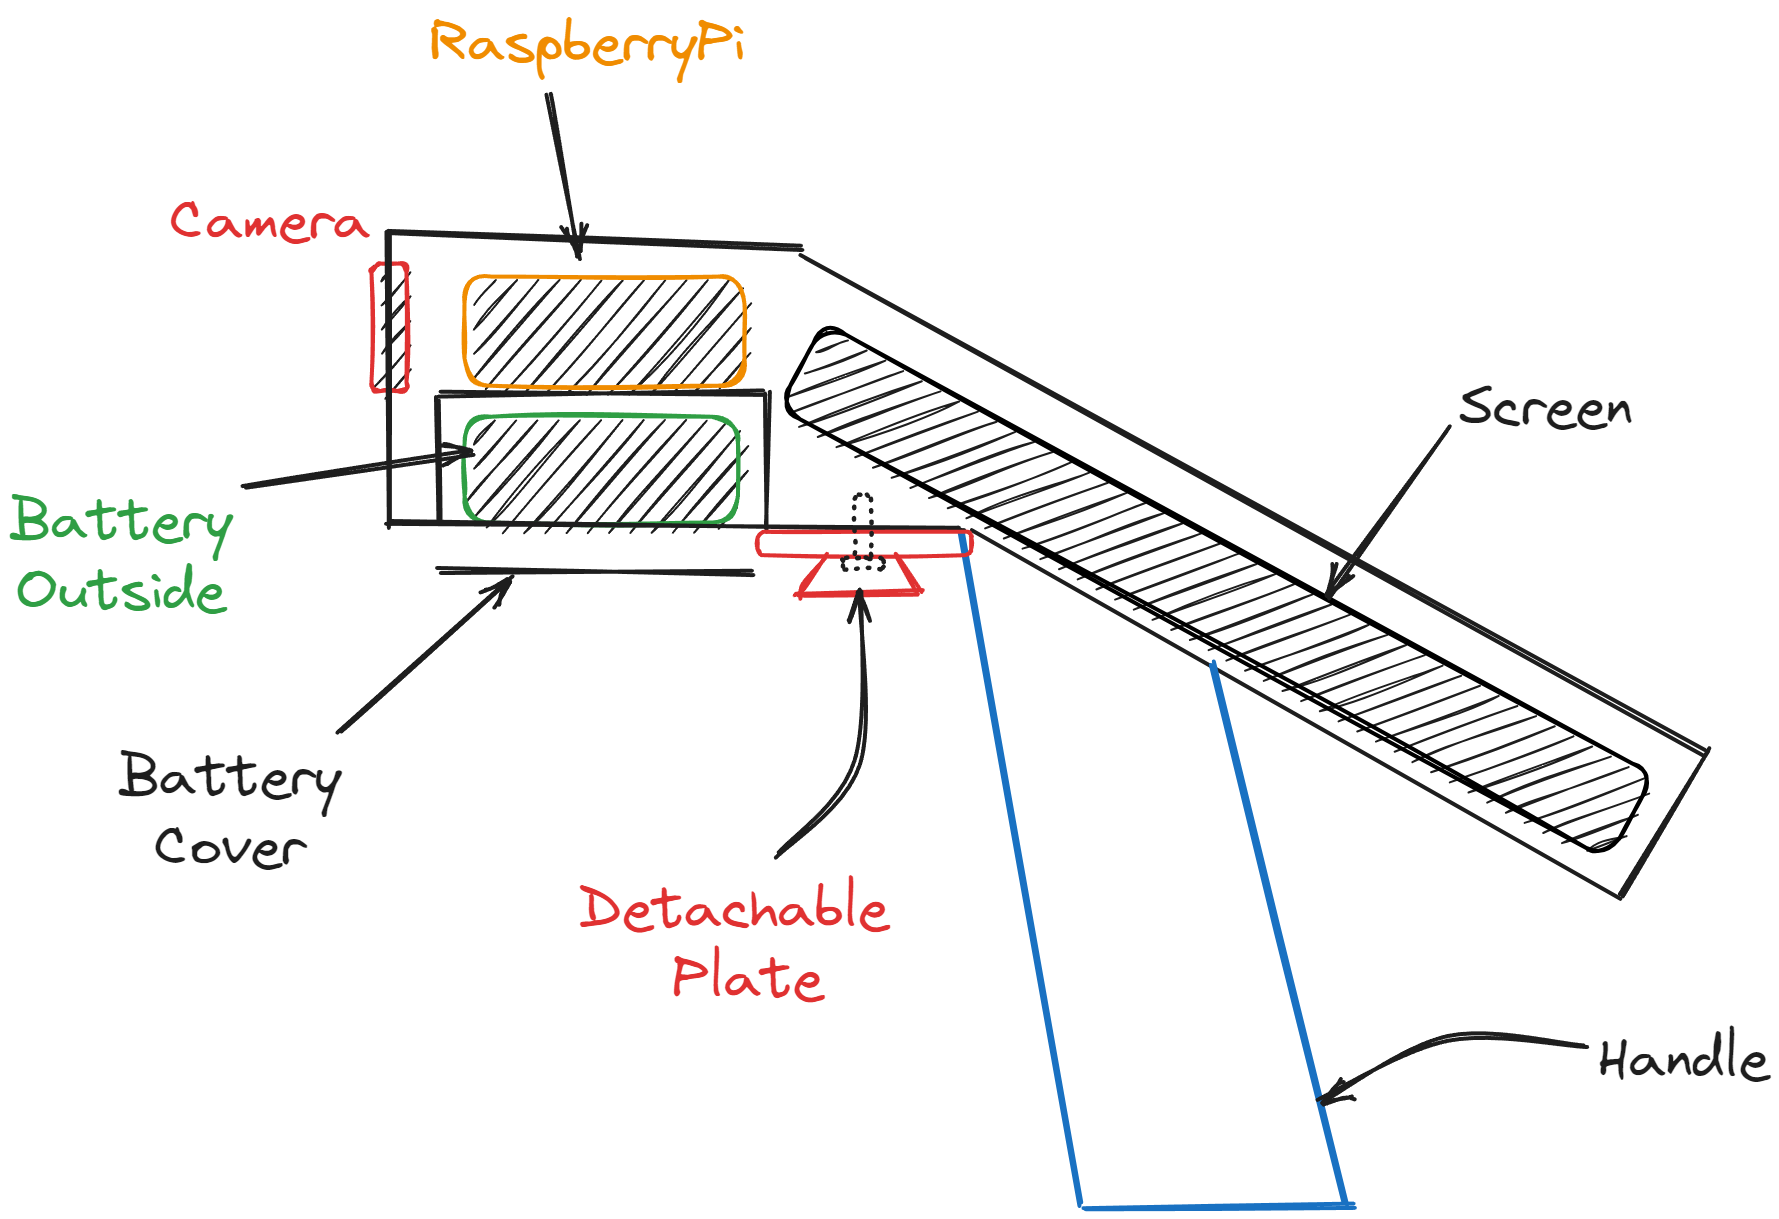
\includegraphics[width=\linewidth]{texs/Part1/chapter3/image/v6.png}
    \caption{Sketch of Solution Variant 6}
    \label{fig:sketch-solution-variant-6}
\end{figure}

The screen orientation remains in portrait mode, providing a vertical display view.

For handling, the device is equipped with a pistol handle, allowing users to hold and operate it with a firm and ergonomic grip.

The battery is placed externally, and a power bank is used in this variant. This setup offers the convenience of easy battery replacement and ensures extended usage periods.

The chassis type in Solution Variant 6 adopts a bowl-like design, with a main body where all components are attached, and a top cover provides protection and encloses the setup securely.

The mounting tripod system is detachable, facilitating easy attachment and detachment from a tripod stand.

As with the other variants, the control mechanism relies on a touch screen, offering an intuitive and user-friendly interface for interacting with the device's functionalities.

\subsection{Solution Variant 7}

Solution Variant 7 presents a Handheld PC-like component placement, where the screen and battery are aligned, and the Raspberry Pi is positioned behind the screen.

\begin{figure}[ht!]
    \centering
    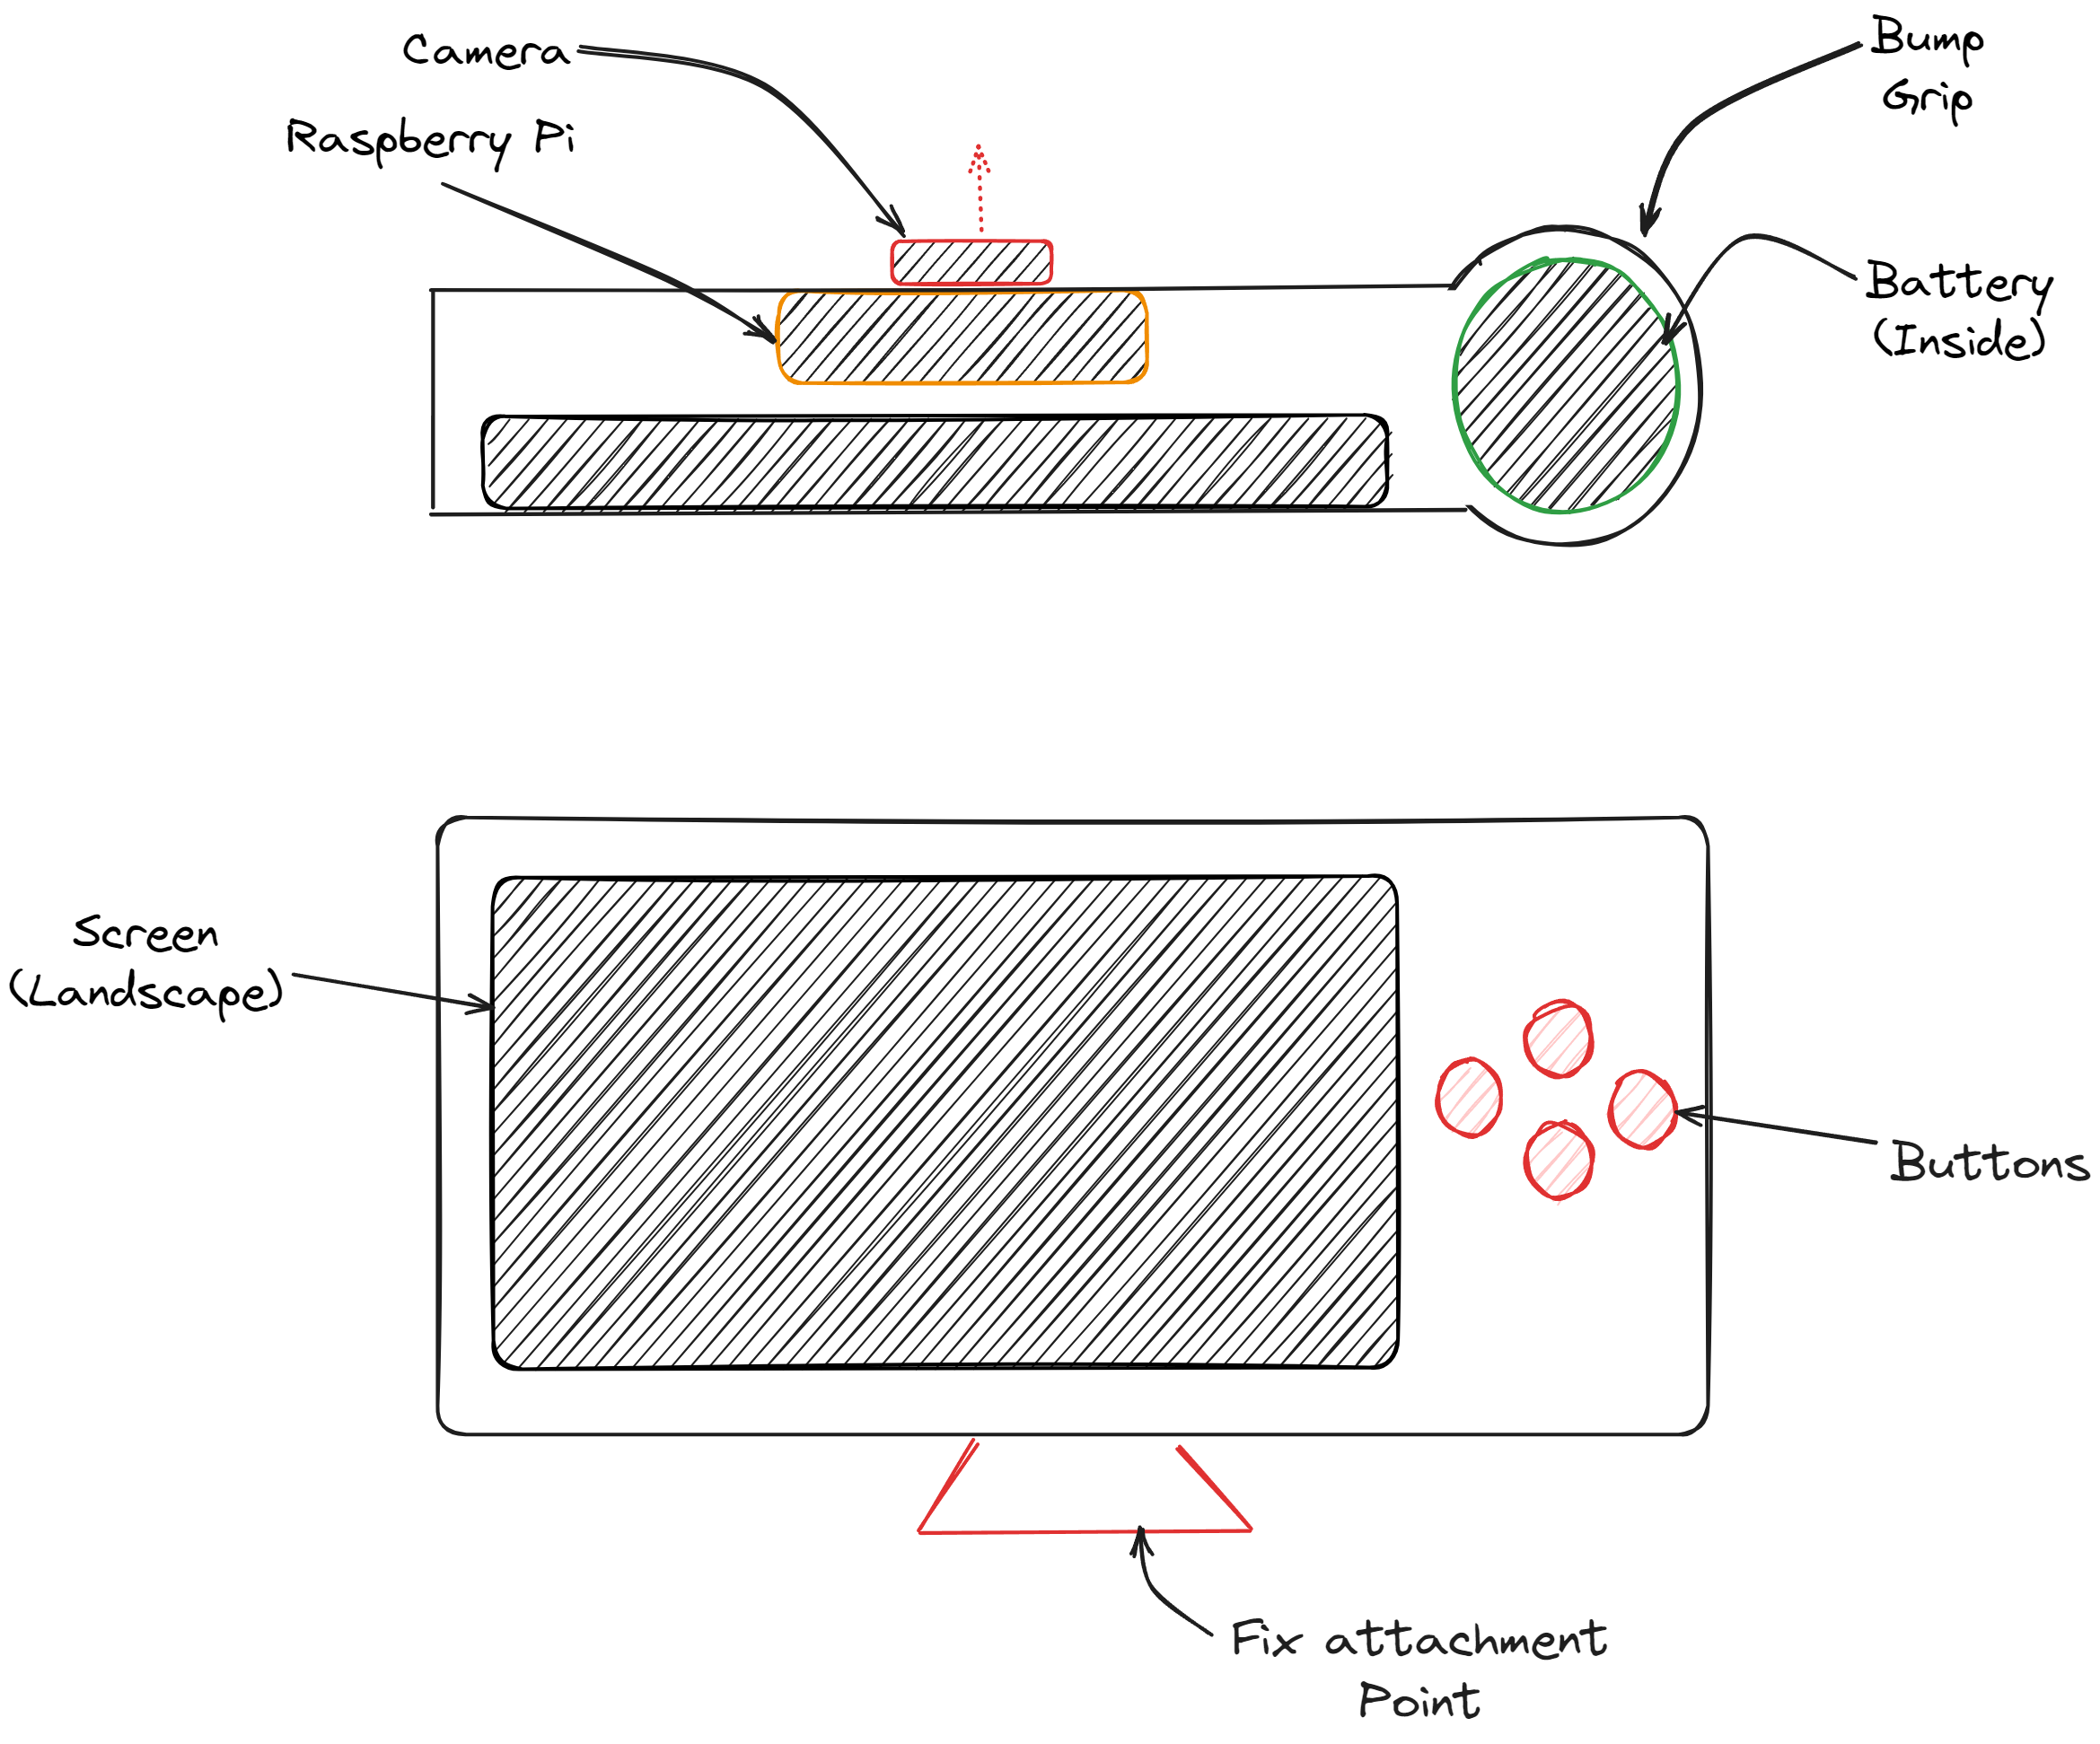
\includegraphics[width=\linewidth]{texs/Part1/chapter3/image/v7.png}
    \caption{Sketch of Solution Variant 7}
    \label{fig:sketch-solution-variant-7}
\end{figure}

The screen orientation is set in landscape mode, offering a wider and horizontal display view.

For handling, the device is designed with a bump grip, providing users with a comfortable and secure way to hold and operate the device.

The battery is placed internally in this variant, and a battery pack is used to power the device, ensuring an integrated and seamless appearance.

The chassis type adopts a bowl-like design, providing a secure enclosure for all components, safeguarding them from potential damage.

For mounting purposes, the device employs a detachable tripod system, making it convenient to attach and detach from a tripod stand.

The control mechanism in Solution Variant 7 combines both a touch screen and physical buttons, providing users with multiple input options for interacting with the device's functionalities. This combination enhances versatility and usability in various scenarios.

\subsection{Solution Variant 8}
Solution Variant 8 features a Camcorder-like component placement, with the Raspberry Pi, Battery, Camera, and Screen arranged similarly to that of a camcorder. The screen is placed at a hinge, allowing it to change angles for flexible viewing.

\begin{figure}[ht!]
    \centering
    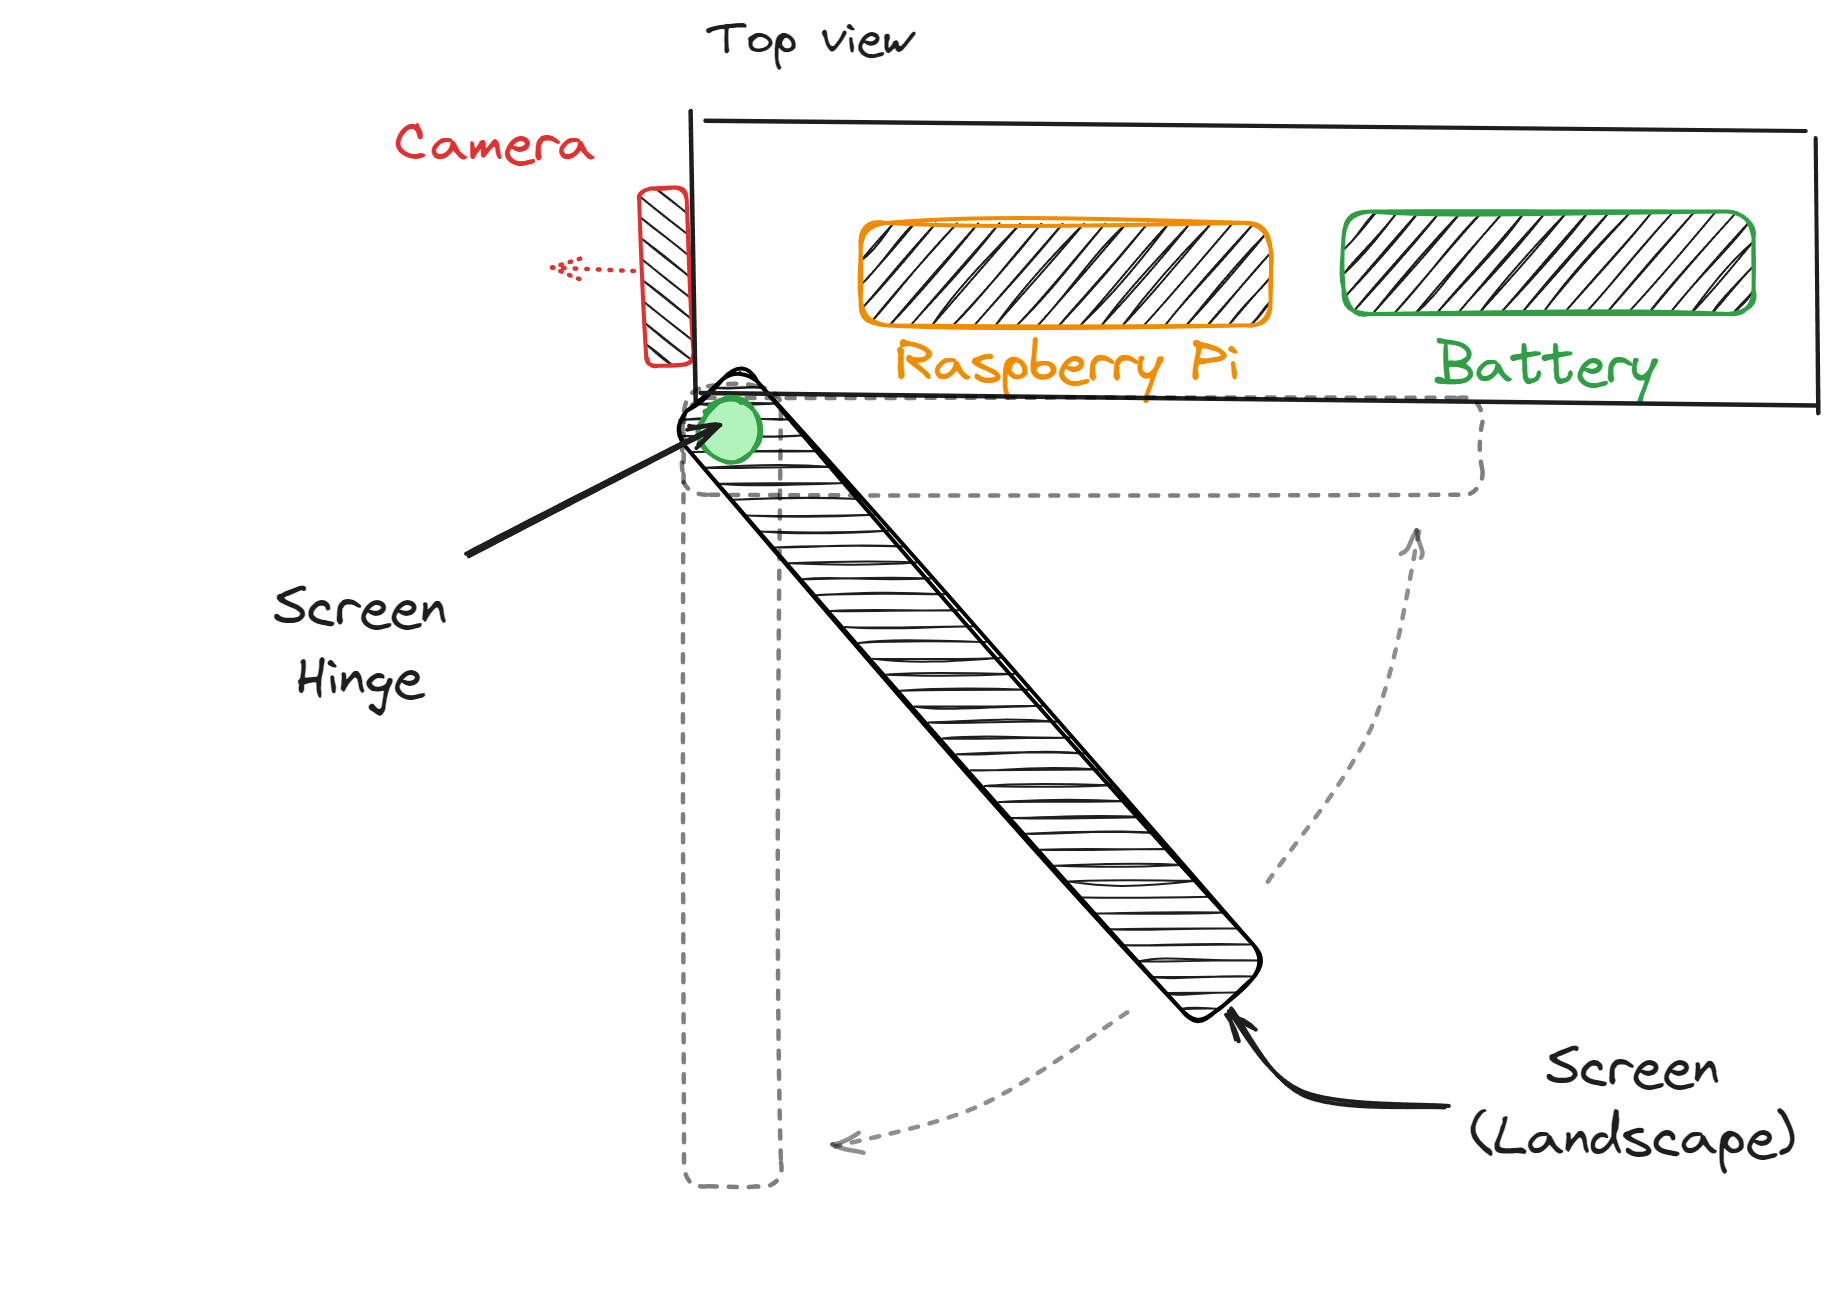
\includegraphics[width=\linewidth]{texs/Part1/chapter3/image/v8.png}
    \caption{Sketch of Solution Variant 8}
    \label{fig:sketch-solution-variant-8}
\end{figure}

The screen orientation remains in landscape mode, providing a wide and horizontal display view.

For handling, the device is designed with a body grip, ensuring a secure and comfortable hold during operation.

The battery is placed internally, and a power bank is utilized in this variant to provide a reliable power source for the device.

The chassis type follows a bowl-like design, offering a protective and sturdy enclosure for all components.

For mounting, a fixed mount tripod system is used, providing stability and ease of use when attaching the device to a tripod stand.

The control mechanism combines both a touch screen and physical buttons, allowing users to interact with the device's functionalities through intuitive touch commands or precise button inputs, offering enhanced control and flexibility in various situations.

\section{Filtering of Solution Variants}

The filtering process is conducted to select the most suitable solution variant for the project. The filtering criteria are based on the design requirements and the design objectives.

\begin{figure}[ht!]
    \centering
    {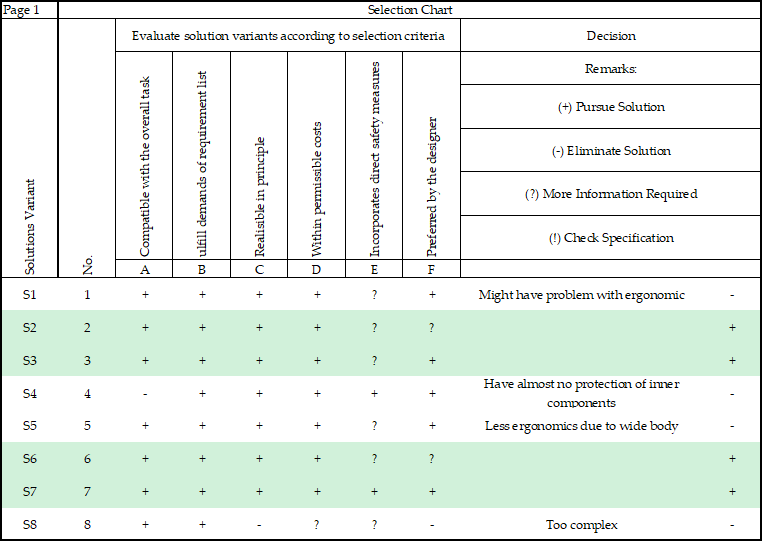
\includegraphics[width=\linewidth]{texs/Part1/chapter3/image/selchart2.png}}
    % \fcolorbox{white}{black}{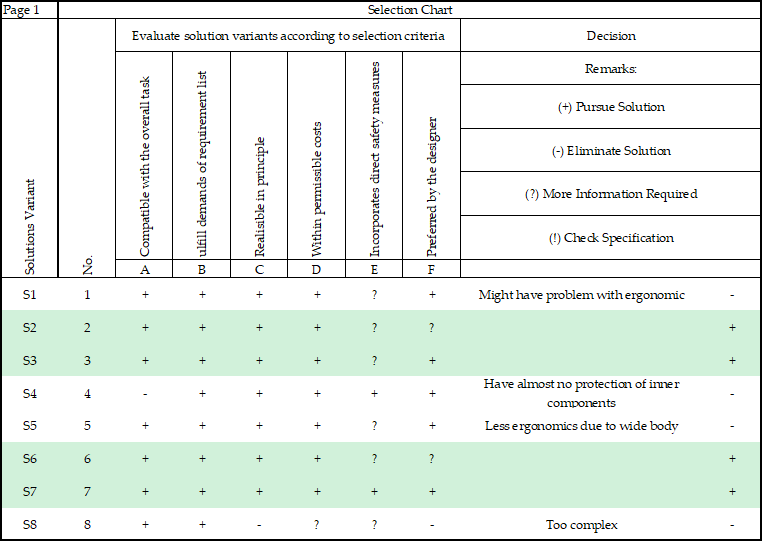
\includegraphics[width=\linewidth]{texs/Part1/chapter3/image/selchart2.png}}
    \caption{Selection Chart for Solution Variants}
    \label{fig:selection-chart-solution-variants}
\end{figure}

As can be seen from the selection chart in Figure \ref{fig:selection-chart-solution-variants}, the solutions S1, S4, S5 and S9 are eliminated and will not be considered for the next stage of the design process.

